\chapter{A Dual Chamber Pacemaker Specification}
\begin{itemize}
	\item What are the basic functions?
    \item What happens if new functionalities are applied to the basic model?
\end{itemize}

\section{Basic 5 timing cycles}
\begin{figure}[!b]
\center
%\vspace{-10pt}
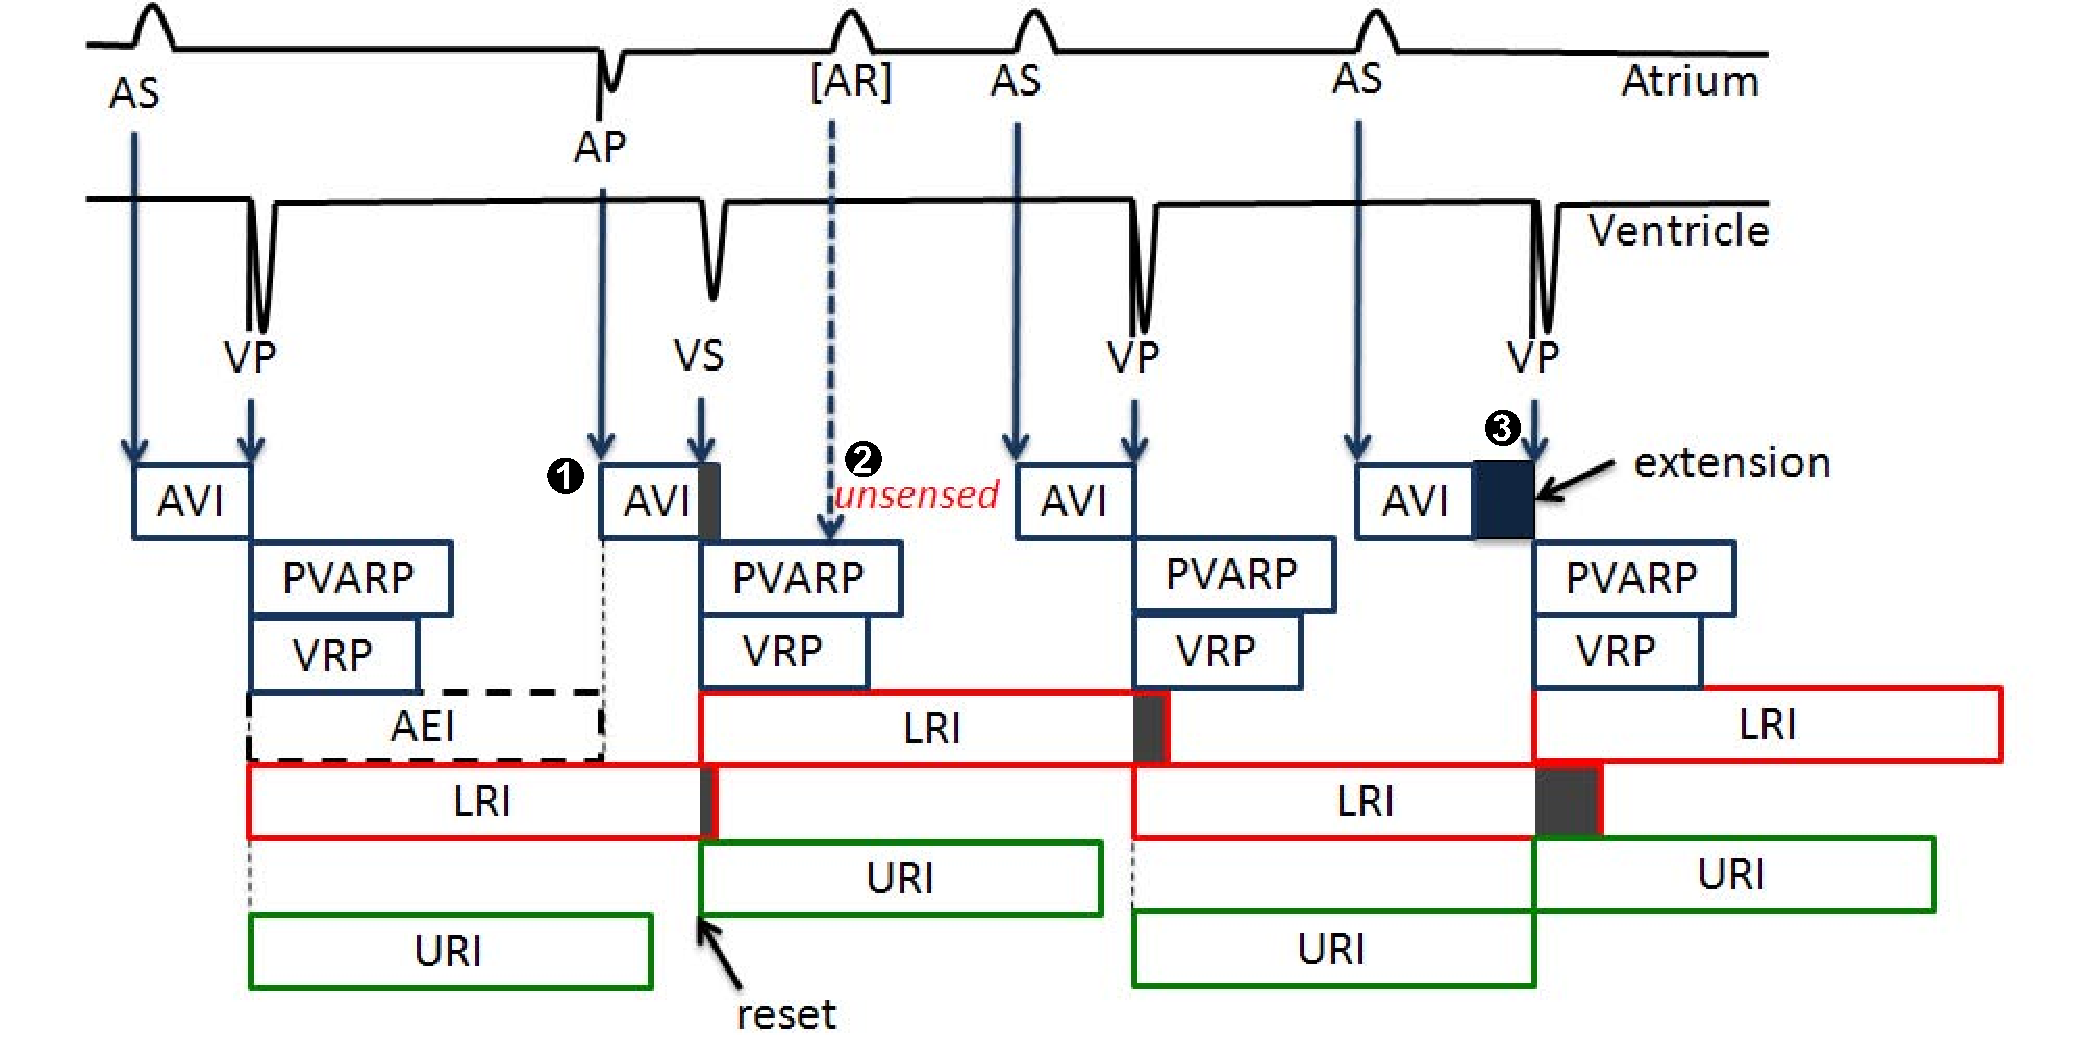
\includegraphics[width=0.7\textwidth]{figs/PM_timers.pdf}
%\vspace{-10pt}
\caption{Basic 5 timing cycles for a dual chamber pacemaker}
\label{fig:PMtimers}
%\vspace{-10pt}
\end{figure} 
\section{Atrial Tachycardia Response (Mode Switch)}
\begin{figure*}[!t]
\centering
		\subfigure [\small]{			
		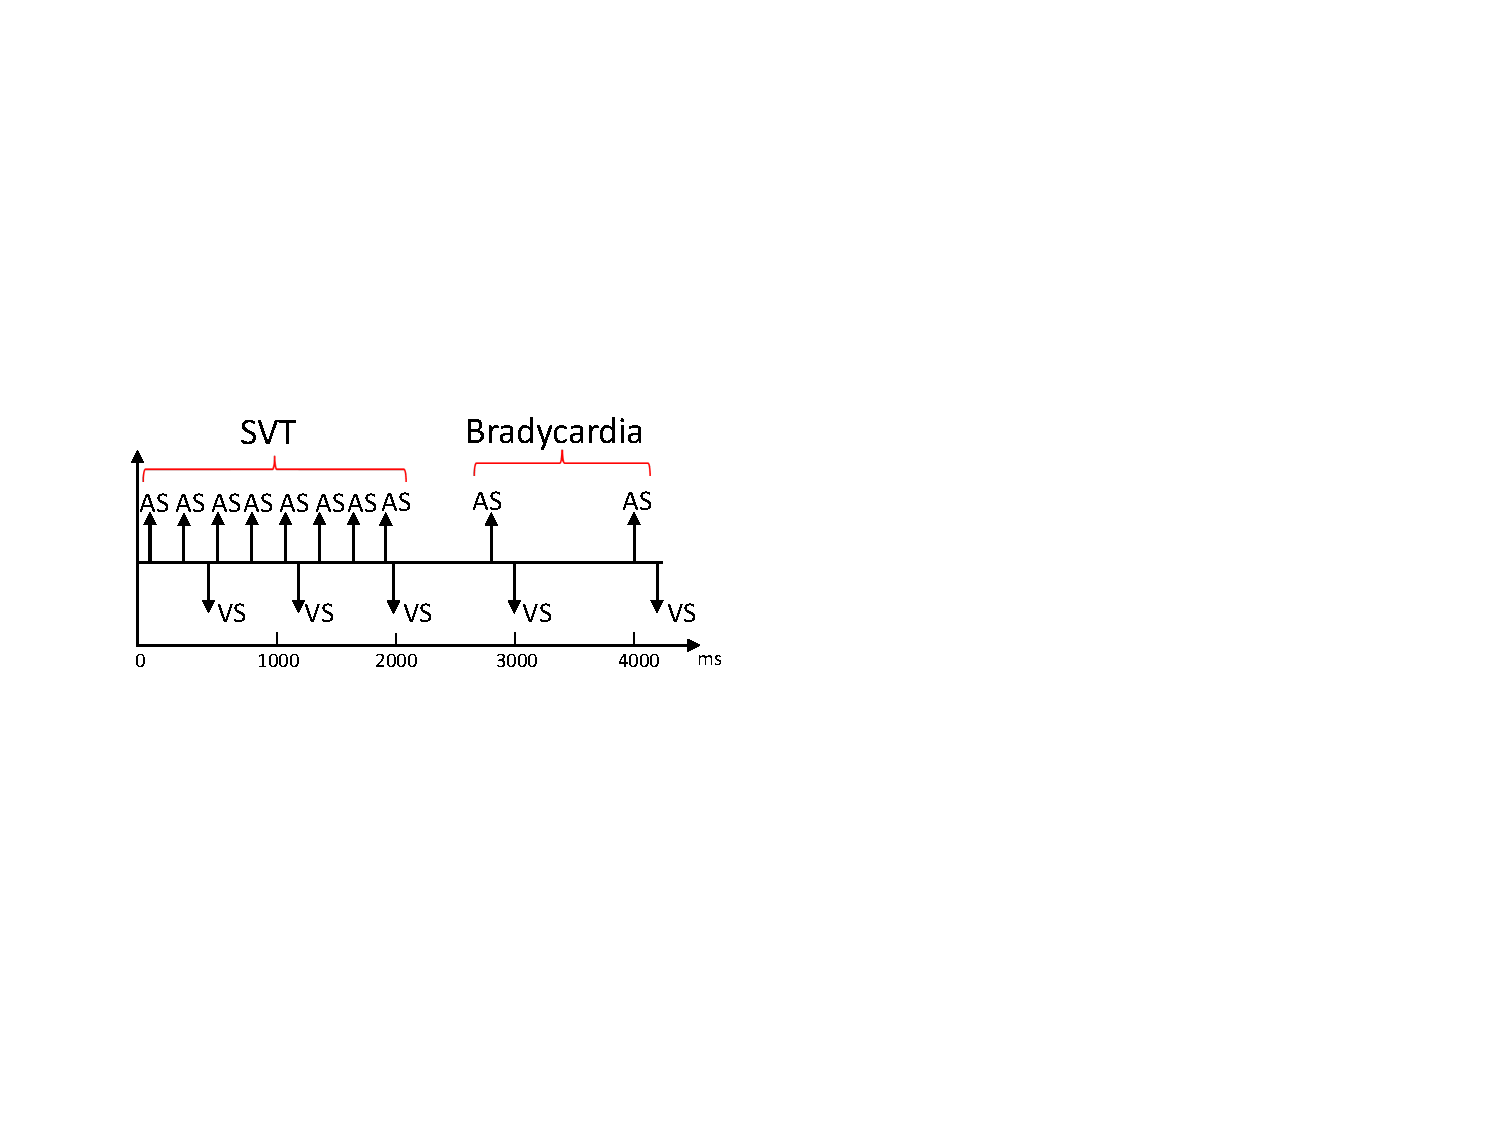
\includegraphics[width=0.4  \textwidth]{figs/SVT_none.pdf}
		\label{fig:SVT_none}
		} 
%	\hspace{.1in}%
		
		\subfigure [\small] 
		{
		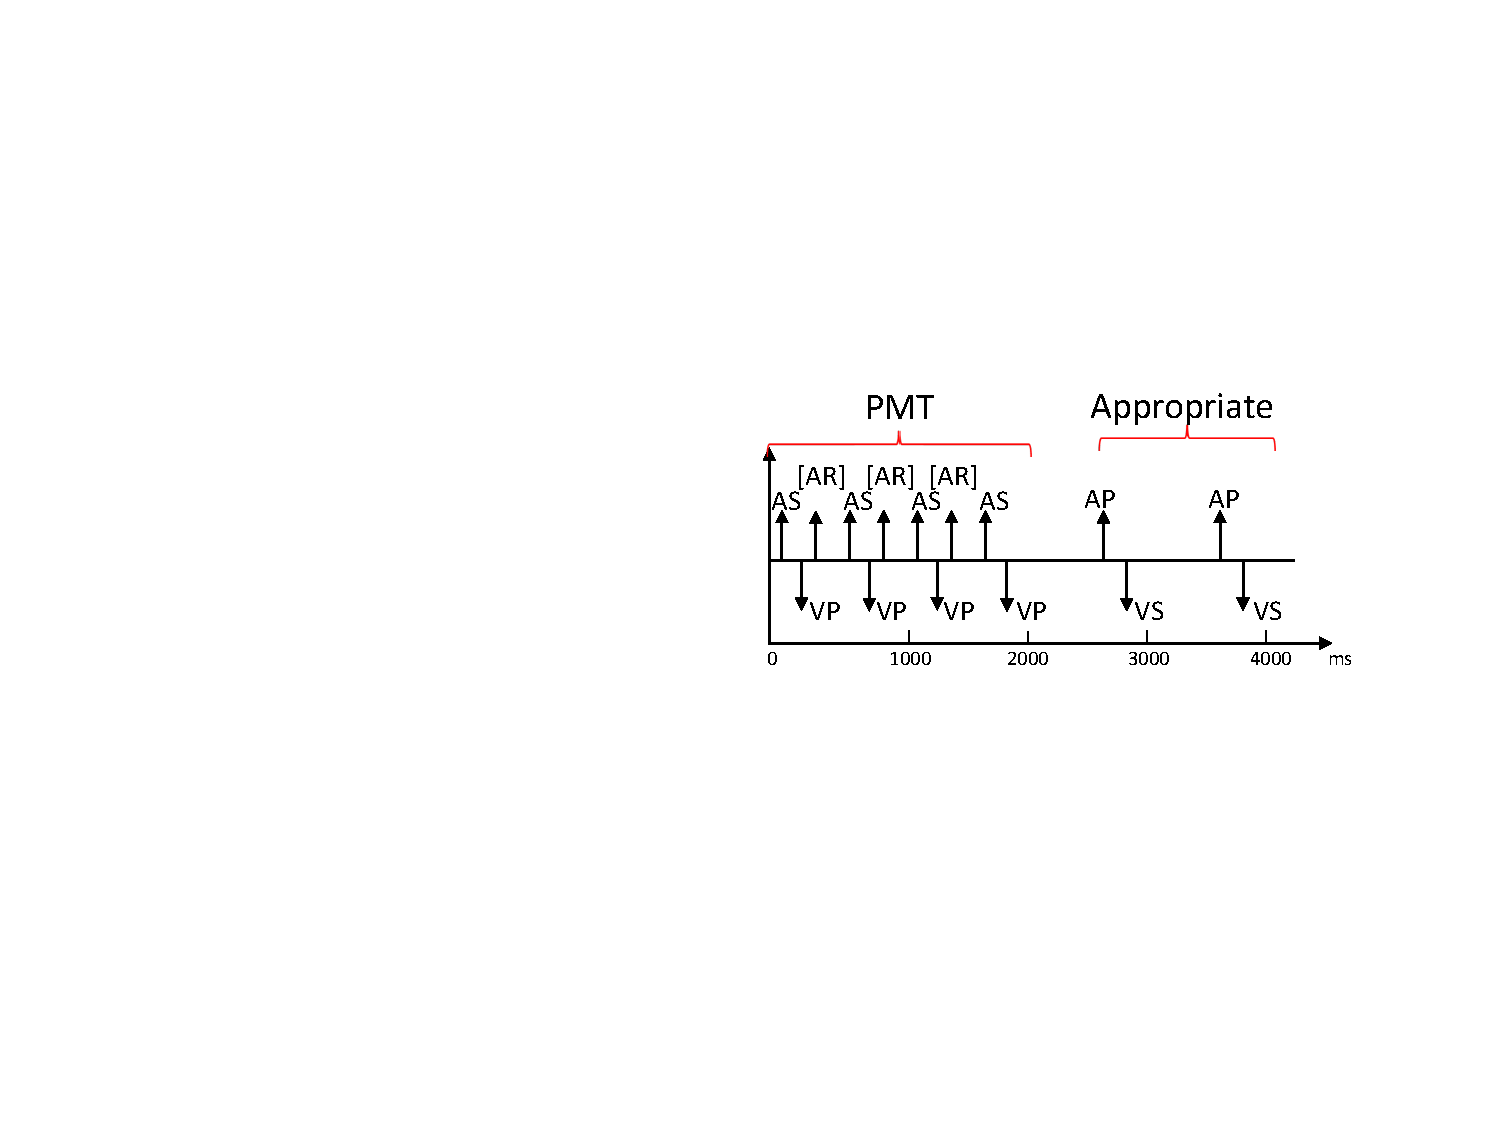
\includegraphics[width=0.4\textwidth]{figs/SVT_DDD.pdf}
		\label{fig:SVT_DDD}
		} 
%\vspace{-10pt}
\caption{\small (a) Node automaton. Dotted transition is only valid for pacemaker tissue like SA node; (b) Path automaton; (c) Model of the electrical conduction system of the heart using a network of node \& path automata~\cite{vhm_ecrts10}.}
%\vspace{-15pt}
\end{figure*} 

\section{Pacemaker Mediated Tachycardia Termination}
show need for closed-loop. open-loop inputs of this scenario

\begin{figure*}[!t]
\centering
		\subfigure [\small]{			
		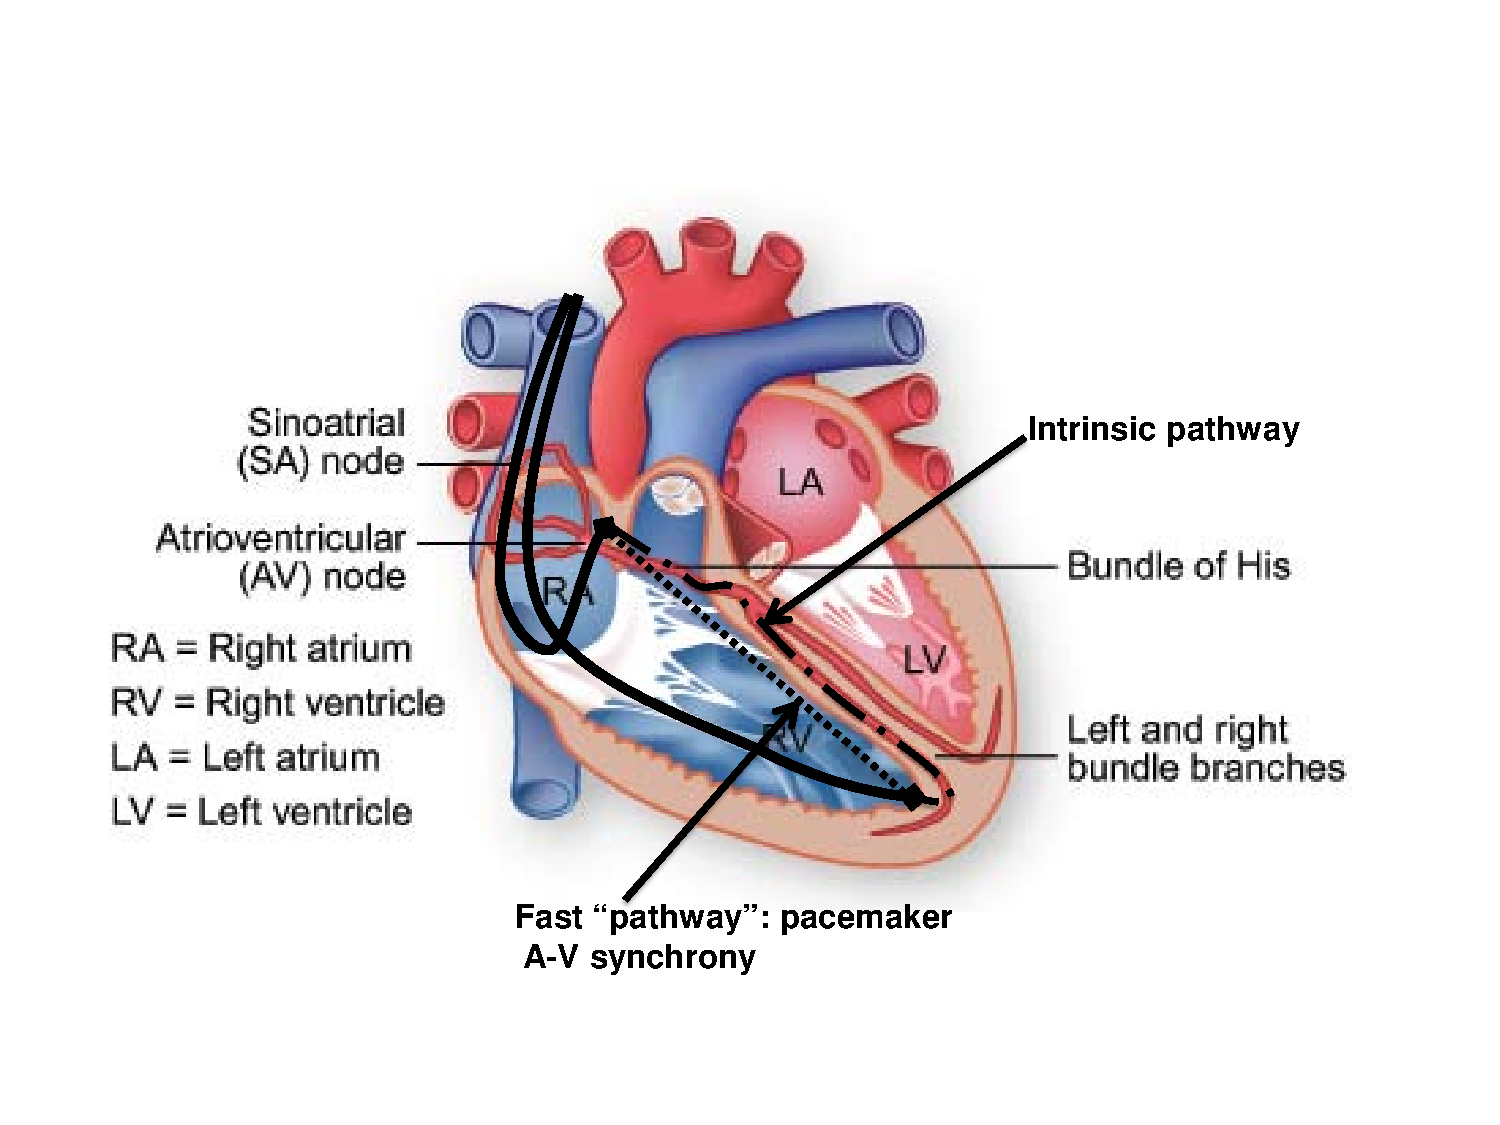
\includegraphics[width=0.4  \textwidth]{figs/ELT_str.pdf}
		\label{fig:ELT_str}
		} 
%	\hspace{.1in}%
		
		\subfigure [\small] 
		{
		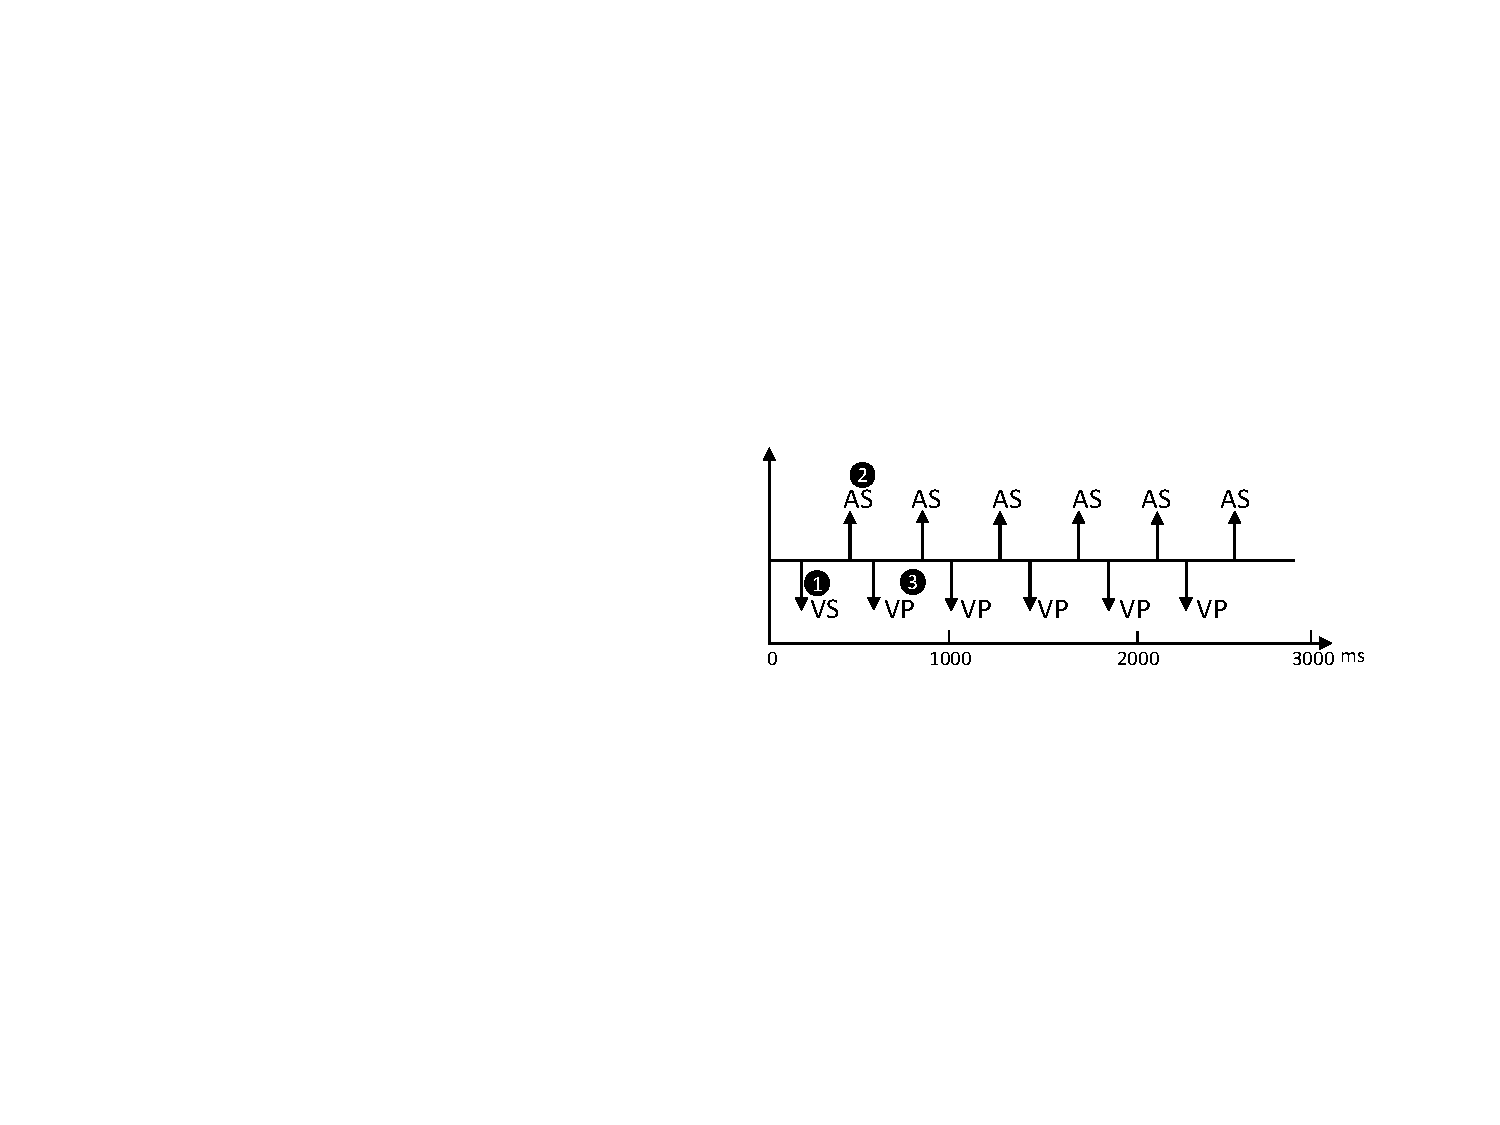
\includegraphics[width=0.4\textwidth]{figs/ELT.pdf}
		\label{fig:ELT}
		} 
%\vspace{-10pt}
\caption{\small (a) Node automaton. Dotted transition is only valid for pacemaker tissue like SA node; (b) Path automaton; (c) Model of the electrical conduction system of the heart using a network of node \& path automata~\cite{vhm_ecrts10}.}
%\vspace{-15pt}
\end{figure*} 


\chapter{Closed-loop Model Checking}
\begin{itemize}
	\item How to use models to cover environmental conditions specified in the physiological requirements, that the device may encounter?
            \item What are the physiological requirements? What form should they be?
            \item Can model checking find violations that testing cannot find?
            \item What are the effects of adding new features? Can they disrupt the safety properties that the previous device hold?
            \item What is the model complexity requirements for each physiological requirement? When and how to refine the environment model?
            \item Exploring the whole state space sounds great. What are the limitations of model checking? 
\end{itemize}

\section{Basic Requirements}
\section{Advanced Functions}
\subsection{Atrial Tachycardia Response}
\subsection{Endless Loop Tachycardia}
\section{Heart Model Refinements}
    
\section{Quantitative Model Checking}

\chapter{Closed-loop Model Simulation/Testing}
\begin{itemize}
	\item What are the limitations of model checking?
    \item How can simulation complement that?
\end{itemize}

\section{Crosstalk}

\section{Lead Displacement}
